
\begin{frame}
	\frametitle{Demodulation}
	\centering 
\includegraphics[scale=.5]{images/gnuradio_logo.png}

	\begin{columns}[c] % align columns
		\begin{column}{.48\textwidth}
			\begin{block}{GNUradio}
				\begin{itemize}
					\item Free and Open-source Software
					\item Software Radio
					\item Signal Processing
				\end{itemize}
			\end{block}
		\end{column}%
		\hfill%
		\begin{column}{.48\textwidth}
			\begin{block}{Configuration}
				\begin{itemize}
					\item Sample Rate 
					\item Frequency
					\item Period
					\item Gain
				\end{itemize}
			\end{block}
		\end{column}%
	\end{columns}
\end{frame}

\begin{frame}
	\frametitle{Raw Signal}
	\centering 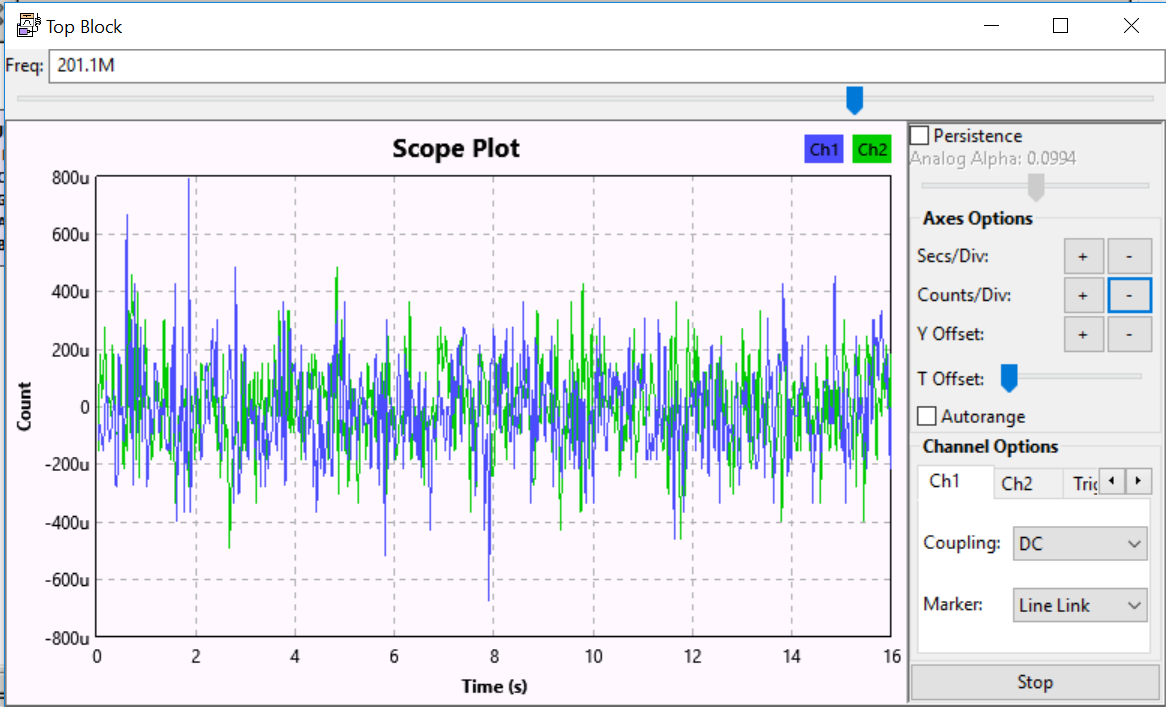
\includegraphics[scale=.35]{images/raw_sig.png}
	\begin{block}{Source Output}
		\begin{itemize}
			\item Complex Signal:
			\begin{itemize}
				\item In-phase 
				\item Quadrature
			\end{itemize}
			\[s(t)=i(t)+jq(t)=r(t).e^{j\varphi(t)} \]
		\end{itemize}
	\end{block}
\end{frame}

\begin{frame}
	\frametitle{Instantaneous Power}
	\centering 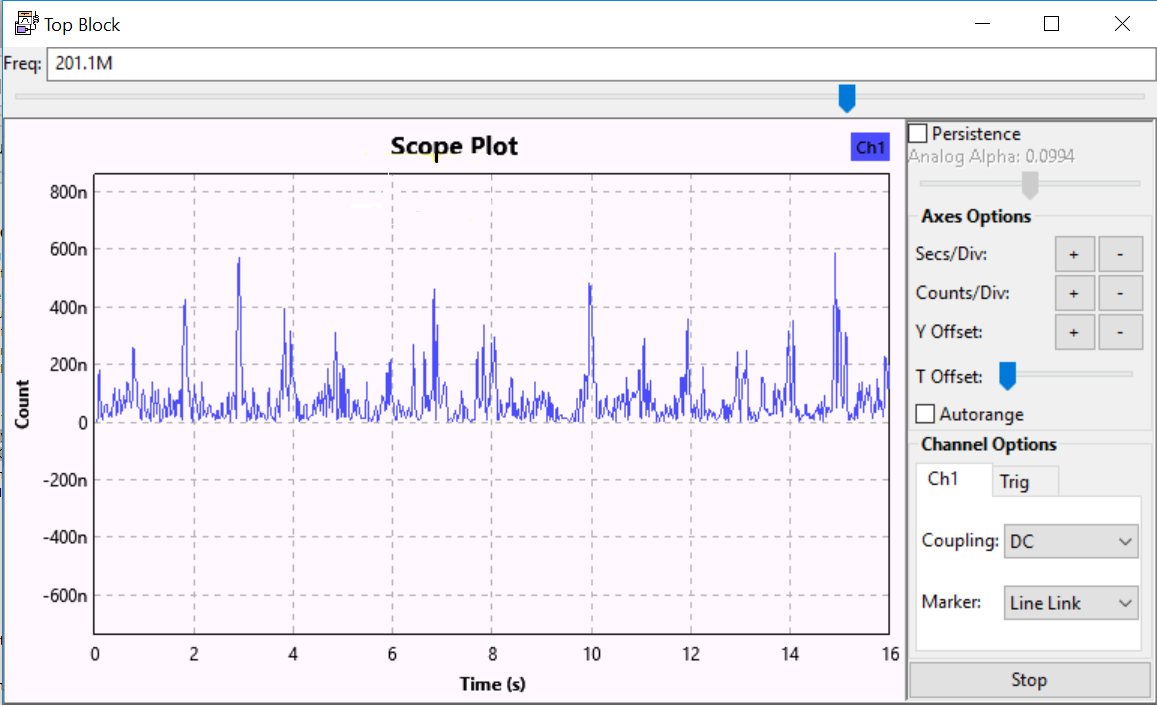
\includegraphics[scale=.35]{images/apres_mag2.png}
	\begin{block}{Float Signal}
		\begin{itemize}
			\item Amplitude
			\item Magnitude
			\[P(t)=|r(t)|^2\]
		\end{itemize}
	\end{block}
\end{frame}

\begin{frame}
	\frametitle{Sliding Average}
	\centering 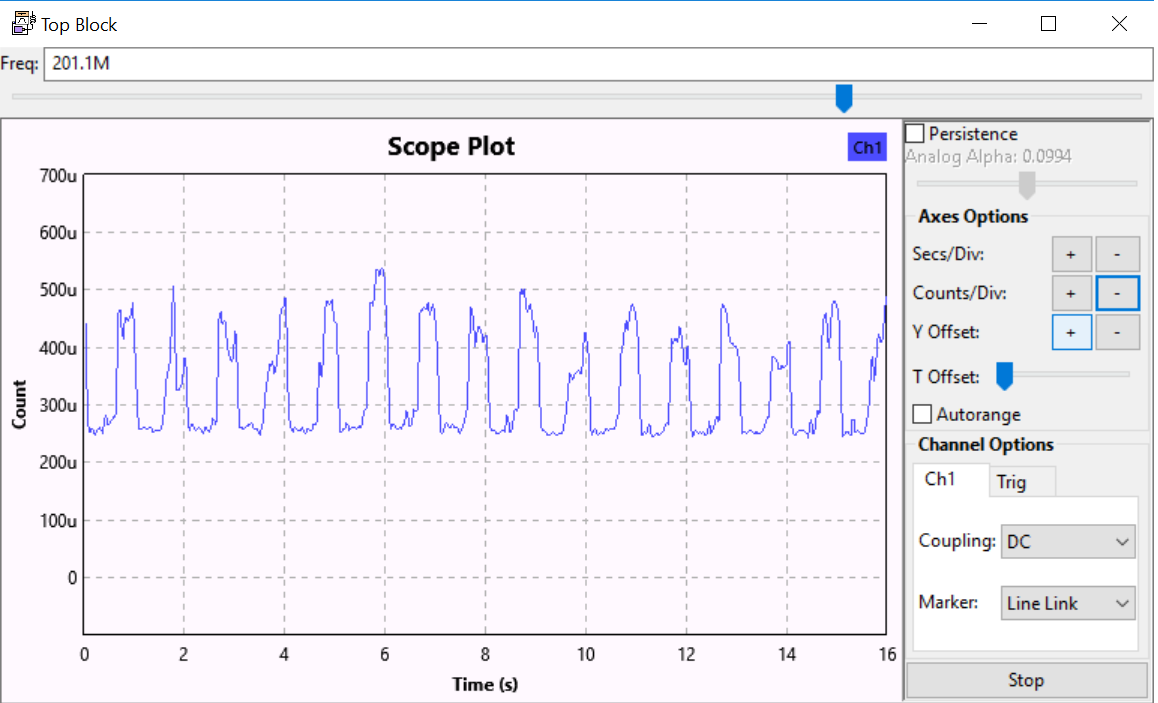
\includegraphics[scale=.35]{images/apres_average.png}
	\begin{block}{Float Signal}
		\begin{itemize}
			\item Number of samples
			\item Treshold
		\end{itemize}
	\end{block}
\end{frame}

\begin{frame}
	\frametitle{Signal Before Decision}
	\centering 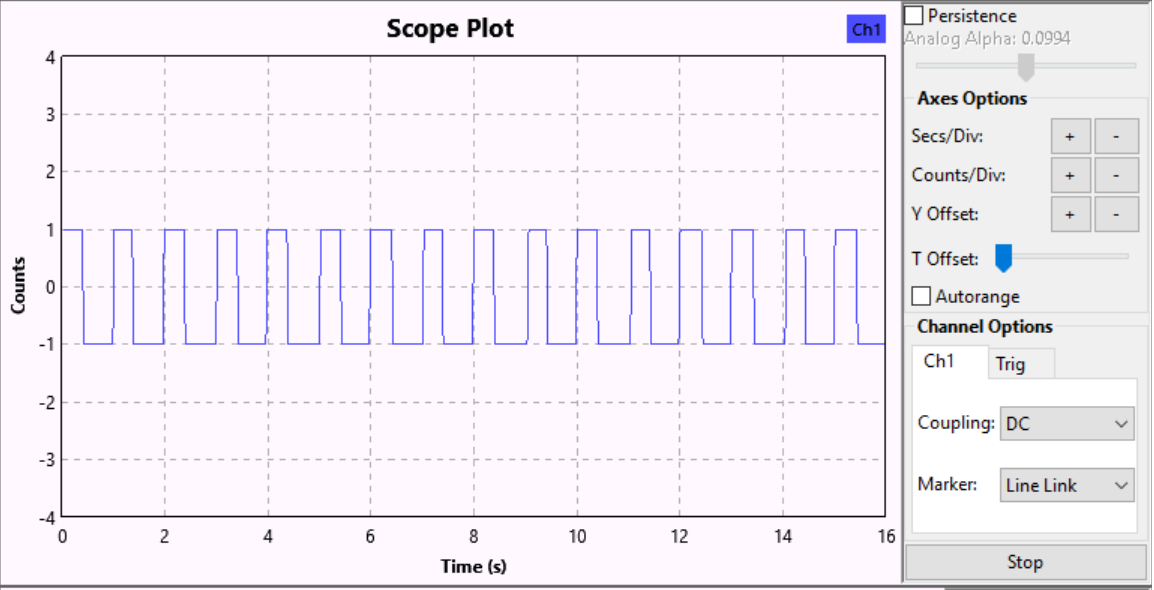
\includegraphics[scale=.35]{images/apres_add_const.png}
	\begin{block}{Square Wave}
		\begin{itemize}
			\item Clock period
			\item Output Byte
			\item Byte Processing
		\end{itemize}
	\end{block}
\end{frame}

\begin{frame}
	\frametitle{Signal processing}
	\begin{block}{Things to improve}
		\begin{itemize}
			\item Noise
			\item Synchronization
			\item Transmitter
			\item BER
		\end{itemize}
	\end{block}
\end{frame}
